\chapter{Design Concept and Rationale}
\label{chap:design}

The \textit{RotaSense} is a device that can track the degree to which the user
turns their head and relay this data to the other components of the take-home
kit. The \textit{RotaSense} is intended to be mounted on the \textit{Blinky} (the
glasses), and sends data to \textit{LeftAware} (the mobile app), the
\textit{Blinky} and the \textit{TheraPulse} (the haptic clip). The design has
an accelerometer gyroscope that is able to track how far and how quickly the
user is turning their head. This data is processed by the ESP32
microcontroller, and then relayed to the other components using
the communication protocols. 

The following sections describe the components of the
device --- accelerometer/gyroscope, ESP32 microcontroller, and communication
protocols --- as well as the rationale for each component.

\section{Accelerometer/Gyroscope}\label{sec:mpu6050}

When creating this device, we needed some way of tracking movement and some way
of processing the movement data and communicating it with the app. In order to
track the users’ movement, we decided to use a MPU6050 Six-Axis Gyroscope and
Accelerometer. This device was chosen due to its simplicity, affordability, and
library support.

The MPU6050 is a commonly used gyroscope/accelerometer. It features high
resolution motion tracking with a built-in Digital Motion Processor to allow for
high-resolution data capture ($\pm 2g$) with data-processing on chip. This
allows us to capture high-quality head position data with minimal power draw and
computing resources on the microcontroller. The MPU6050 is also very small
(smaller than a fingernail), lightweight (less than \qty{5}{\g}), and affordable
(costing around \$3 for a development board). And most importantly, it is a very
easy to use device with excellent library support through I2CDevLib on the
Arduino framework, allowing us to quickly prototype, test, and iterate on our
design.

\begin{figure}[h]
  \centering
  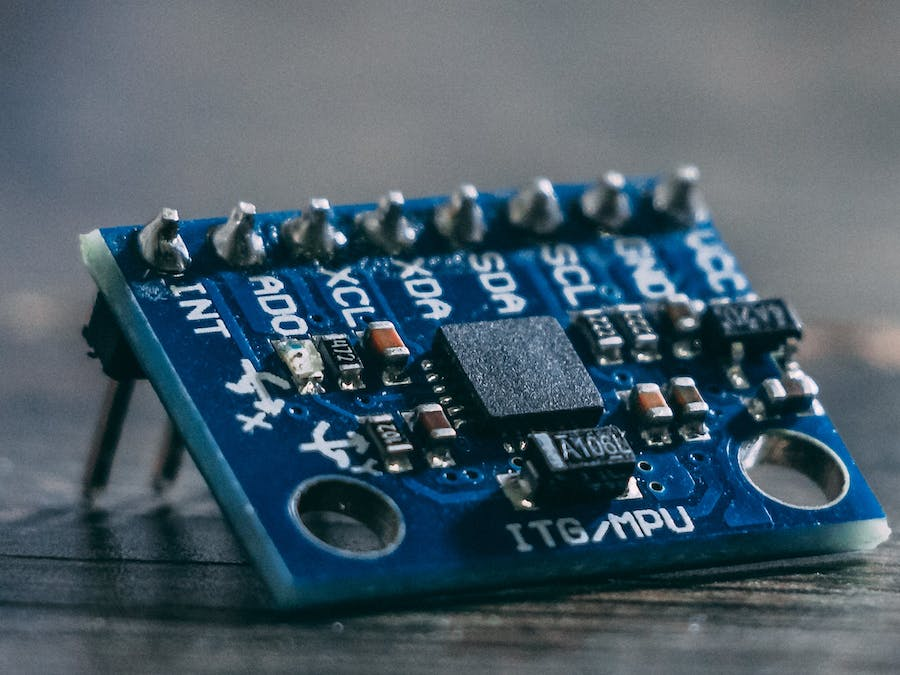
\includegraphics[width=0.3\textwidth]{mpu6050}
  \caption{The MPU6050 Accelerometer and Gyroscope.}
\end{figure}

\section{ESP32 Microcontroller}

For communication purposes, we decided to use the ESP32 microcontroller from
Espressif Systems. This microcontroller is relatively small, with a length of 48
mm, a width of 25 mm, and a height of 11 mm. It supports
Bluetooth 5.0 (Low Energy) and the $I^2C$ communication protocol, which are needed
for talking to the phone and MPU6050 (\autoref{sec:mpu6050}), respectively. It
has two cores that can run at up to 240 MHz, a deep sleep mode for extremely low
power consumption, and a large online support base to allow for easy
development. The chip is powerful enough to run a lightweight operating system,
so we are able to use multiple processes to speed up computation and also save
energy.

\begin{figure}[h]
  \centering
  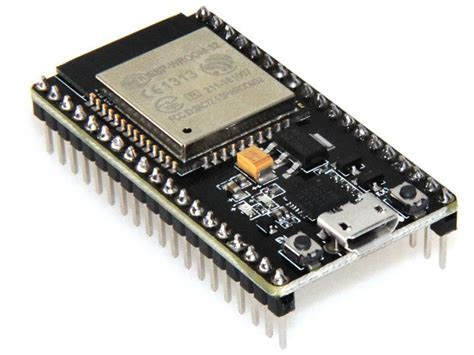
\includegraphics[width=0.3\textwidth]{esp32}
  \caption{The ESP32 Microcontroller.}
\end{figure}

\section{Communication Protocols}

One of the most important components of our design are the communication
protocols.

The I2C communication protocol was chosen due to its simplicity and
unobtrusiveness, requiring only four wires for inter-device communication. It is
a synchronous\footnote{All devices agrees on when messages are sent.}
serial\footnote{Only one message is sent at a time.} communication protocol,
widely used for attaching low-speed peripheral devices (chips) to a controller
chip for short-distance communication. Used widely throughout the industry, it
has great library and device support, with no downsides.

Bluetooth Low-Energy was chosen for its lower energy consumption, as our device
should be able to run for long periods of time while on battery power. While
Bluetooth Low-Energy is a more complex system to work with, introducing more
moving ``parts'' and slightly slowing down our iteration speed, as power
consumption is a main requirement of our design, we felt it was a fair
trade-off.

In the same vein of saving energy, we also will try to use the Deep
Sleep mode of the ESP32 to reduce power consumption during idle periods to only
\qty{5}{\uW}.

%%% Local Variables:
%%% mode: latex
%%% TeX-master: "../final_report"
%%% End:
